\def\ifflag#1{\IfFileExists{./#1.mrp}}

\ifflag{brouillon}{\def\rpModeBrouillon{}}{}

\ifdefined\rpModeBrouillon
	\documentclass[a4paper, oneside, 12pt, draft]{article}
\else
	\documentclass[a4paper, oneside, 12pt]{article}
\fi

%%%%%%%%%% Paquets %%%%%%%%%%

% Paquets pour le Français
\usepackage[utf8]{inputenc} % Gestion encodages
\usepackage[T1]{fontenc} % ???
\usepackage[francais]{babel} % Typographie française

% Divers
\usepackage[noabbrev]{cleveref}
\usepackage{url}
\usepackage{here}
\usepackage{enumitem}

% Images
\usepackage{graphicx}

% Mise en page
\usepackage{geometry}
\parskip=12pt

\usepackage{setspace}
\newenvironment{rmskip}{\bgroup\parskip=8pt\setstretch{1.0}}{\egroup}

\usepackage{color} % Utilisé par \todo

% Tabulations verbatim
% http://www.grappa.univ-lille3.fr/FAQ-LaTeX/6.16.html
\makeatletter
{\catcode`\^^I=\active
\gdef\verbatim{\catcode`\^^I=\active\def^^I{\hspace*{4em}}%
\@verbatim \frenchspacing\@vobeyspaces \@xverbatim}}
\makeatother

%%%%%%%%%% Commandes supplémentaires %%%%%%%%%%%

% Marquage du travail restant
% [#1] Texte à afficher
\newcommand{\todo}[1][Il y a là encore des choses à écrire !]{\colorbox{yellow}{#1}}

%%% Gestion du sommaire
% Section non numérotée
% {#1} Nom de la section
\newcommand{\sectionSpeciale}[1]{\section*{#1}\addcontentsline{toc}{section}{#1}}
% Section non numérotée dont le titre n’est pas affiché.
% {#1} Nom de la section
\newcommand{\sectionCachee}[1]{\addcontentsline{toc}{section}{#1}}

%%% Gestion des annexes
\makeatletter
	
	\newcounter{annctr}
	
	% Définir une annexe
	% {#1} Nom de l’annexe
	\newcommand{\annexe}[1]{\stepcounter{annctr}\addcontentsline{ann}{section}{\protect\numberline {\Alph{annctr}}#1}\section*{\numberline {\Alph{annctr}}#1}}
	% Lister les annexes
	% Note : ce serait quand même bien de le faire fonctionner sans avoir besoin du makefile.
	\newcommand\listeannexes{\sectionSpeciale{Annexes}\input{annexes.tex}}
	
	% Déclaration et ouverture du fichier de stockage de la liste des annexes
	\newwrite\tf@ann
	\immediate\openout\tf@ann\jobname.ann\relax
      
\makeatother

%%%%%%%%%% Bibliographie et webographie %%%%%%%%%%

\usepackage{multibib}
\newcites{web}{Références webographiques}

%%%%%%%%%% Abstract %%%%%%%%%%

\newcommand\keywords[2]{%
	\begin{itshape}
		\noindent\textbf{#1} #2
	\end{itshape}
}

%%%%%%%%%% Abstraction de la mise en forme %%%%%%%%%%

\newcommand\nom[1]{\textsc{#1}}
\newcommand\classe[1]{\textit{#1}}

%%%%%%%%%% Outils %%%%%%%%%%

\newcommand\rpFun{{\em{Informatique des Systèmes Embarqués}}}
\newcommand\rpFdeux{{\em{Génie Logiciel et Systèmes Informatiques}}}
\newcommand\rpFtrois{{\em{Systèmes d’Information et Aide à la Décision}}}
\newcommand\rpFquatre{{\em{Calcul et Modélisation Scientifiques}}}
\newcommand\rpFcinq{{\em{Réseaux et télécommunications}}}

%%%%%%%%%% Configuration %%%%%%%%%%

\def\rpTitreLexique{Glossaire}
\def\rpTypeTuteurIsima{Responsable}
\def\rpTypeTuteurEntreprise{Responsable}
\def\rpInterligne{1.5}
\def\rpDossier{contenu}
\def\rpLargeurLogoEntreprise{6cm}

% R�tro-compatibilit�
% Ne pas modifier dans le d�p�t ma�tre, pour �viter d'�craser la configuration
% des d�p�ts l'utilisant.
% R�tro-compatibilit�
% Ne pas modifier dans le d�p�t ma�tre, pour �viter d'�craser la configuration
% des d�p�ts l'utilisant.
\input{contenu/configuration}



\setstretch{\rpInterligne}

%%%%%%%%%% Pied de page %%%%%%%%%%

\usepackage{fancyhdr}
\pagestyle{fancy}
\fancyhf{}
\renewcommand{\headrulewidth}{0pt}

\ifdefined\rpNumeroADroite
	\let\rpPiedPositionNumero\rfoot
	\let\rpPiedPositionConfidentiel\cfoot
\else
	\let\rpPiedPositionNumero\cfoot
	\let\rpPiedPositionConfidentiel\rfoot
\fi

\rpPiedPositionNumero{\thepage}
\ifdefined\rpConfidentiel\rpPiedPositionConfidentiel{\rpConfidentielTexte}\fi



\begin{document}

%%% Page de garde %%%

\begin{rmskip}
	% Pas de numéro sur cette page
\thispagestyle{empty}
\newgeometry{top=2cm, bottom=2cm, left=2cm, right=2cm}

% Note : logo disponibles sur http://fc.isima.fr/~brunot/files/isima/logos/
% J’avais trouvé une version vectorielle, ce serait mieux, mais je ne la trouve plus…
\def\rp@isima{%
	\begin{minipage}[t]{6cm}
		\vspace{0pt}
\includegraphics[width=\rpLargeurLogoIsima]{._tex/isima.png}
		
		\vspace{0.5cm}
		
		\begin{minipage}{4cm}
			\begin{flushleft}
				Institut Supérieur d’Informatique, de Modélisation et de leurs Applications
				
				\vspace{0.5cm}
				
				{\footnotesize 1 rue de la Chebarde \\ TSA 60125 \\ CS 60026 \\ 63178 Aubière CEDEX }
			\end{flushleft}
		\end{minipage}
	\end{minipage}
}

\ifdefined\rpLogoEntreprise{
	\begin{tabular*}{\textwidth}{l @{\extracolsep{\fill}} r}
		{ \rp@isima } & \begin{minipage}[t]{6cm}
			\begin{flushright}
				\vspace{0pt}\includegraphics[width=\rpLargeurLogoEntreprise]{\rpLogoEntreprise}
				
				\vspace{0.5cm}
				
				\begin{minipage}{4cm}\begin{flushright}
					\rpEntreprise
				\end{flushright}\end{minipage}
			\end{flushright}
		\end{minipage}
	\end{tabular*}
}\else{
	\rp@isima
}\fi

\vspace{3cm}

\begin{center}
	Rapport d’ingénieur \\
	{\rpType} de \rpAnnee{\ieme} année \\
	Filière \rpFiliere \\
	\Large{\textbf{\rpTitre}}
\end{center}

\vspace{4cm}

\begin{tabular}{ll}
\textit{Présenté par :} & \textbf{\rpNom} \\
\ifdefined\rpSecondNom
	& \textbf{\rpSecondNom} \\
\fi
 & \\
\textit{{\rpTypeTuteurEntreprise} entreprise :} & \textbf{\rpTuteurEntreprise} \\
\textit{{\rpTypeTuteurIsima} ISIMA :} & \textbf{\rpTuteurIsima} \\
\end{tabular}

\begin{flushright}
\textit{Soutenance le} \textbf{\rpDateSoutenance} \\
\textit{{\rpType} de} \textbf{\rpDuree}
\end{flushright}

\restoregeometry


\end{rmskip}

\newpage
	
%%% Avant-propos %%%
\pagenumbering{roman}

\sectionSpeciale{Remerciements}
% Un ou deux paragraphes de remerciement...

\newpage

\sectionCachee{\listfigurename}
\listoffigures
\newpage

% Pas de titre extérieur au fichier, car il en contient deux.
% La macro \keyword{ -- mot-clé -- } est définie pour les arguments de
% \rpResumeAuto ; elle met en gras et ajoute à la liste des mots-clés
% (séparément pour chacun).

\rpResumeAuto{
	% Ceci me semble le bon endroit pour rédiger un résumé
}{
	% Et ici le même, mais en anglais.
}

\newpage

\begin{rmskip}
	\renewcommand{\contentsname}{Table des matières}
	\sectionCachee{\contentsname}
	\tableofcontents
\end{rmskip}
\newpage

% Sauvegarde du numéro de la page courante
\newcounter{metapage}
\setcounter{metapage}{\value{page}}
% Remise à zéro des numéros de page & changement de chiffres
\pagenumbering{arabic}

%%% Contenu %%%

\sectionSpeciale{Introduction}
% Introduction du rapport

L'Internet des Objets (\textbf{IdO} ou \textbf{IoT} pour \textit{Internet of Things} en anglais) représente la jonction entre Internet et le monde des capteurs qui ne sont généralement pas directement reliés à des équipements actifs des réseaux, comme un routeur par exemple. En effet, usuellement les données passent plutôt par une phase de traitement sur un ordinateur avant d'être potentiellement envoyées sur le réseau.

Tous les concepts derrière l'IoT soulèvent plusieurs problématiques telles que l'accroissement exponentiel du volume de données sur le réseau, dû à l'explosion du nombre d'objets connectés, mais aussi des problèmes de nature énergétiques, car les capteurs sont rarement alimentés en continue via une prise électrique.

C'est pourquoi plusieurs protocoles ont été créés en prenant en compte ces contraintes, l'un d'eux étant \textbf{6LoWPAN}. Il nous fût demandé d'effectuer une étude sur ce protocole car il présente une particularité que son principal concurrent ne possède pas (\textbf{ZigBee}), celle de pouvoir router l'information depuis n'importe quels nœuds (\textit{node} en anglais). Cela ne nous oblige pas à avoir une topologie maître/esclave, mais plutôt un réseau maillé, ce qui permet de couvrir de plus grandes superficies.

Notre projet consista en une étude de 6LoWPAN ainsi qu'à son expérimentation grâce à des cartes achetées par notre tuteur, le but ultime étant de pouvoir router de l'information via n'importe quelle carte. Aussi ce projet était à vocation exploratoire pour préparer d'autres projets sur l'IoT dans les années futures. La question était donc :

\begin{center}
\textbf{\textit{Comment router de l'information grâce à 6LoWPAN ?}}
\end{center}

Pour répondre, nous allons, dans un premier temps, vous présenter plus en détails l'IoT, certains protocoles et bien sûr 6LowPAN. Ensuite nous reviendrons sur le travail technique que nous avons effectués sur les cartes puis nous dresserons un bilan de ce projet.

\newpage

% Corps du rapport
% Remplissez à votre aise, avec \section comme premier niveau de titre.
% Je conseille de faire au minimum un fichier différent par section de premier
% niveau (de préférence au deuxième), puis de les inclure avec `\input`.

% Partie 1 - l'IoT et ses protocoles %

\section{L'IoT et ses protocoles}

Dans cette première partie, nous allons définir plus en détail quelles sont les implications et les spécificités de l'IoT ainsi que de l'approche au niveau des réseaux via la présentation de quelques protocoles et bien évidemment celle de 6LoWPAN.

% Partie 1.1 - l'IoT %

\subsection{L'IoT}

\textit{L'Internet of Things}, que nous appellerons maintenant IoT pour le reste de ce rapport, se traduit littéralement comme l'Internet des Objets, mais qu'est-ce-qu'un objet? Dans le monde de l'IoT les objets peuvent se référer à des biens (comme des meubles ou de l'électroménager), des machines, des véhicules, des immeubles ou bien même à quelque chose d'organique comme un être vivant (Homme ou animal), une plante, des sols (pour les cultures).

Alors la question est : Comment pouvons nous tous connecter ? En effet, comment faire en sorte qu'une plante possède un accès réseau. C'est cela que l'IoT veut définir et représente, une connectivité pour tout.

Mais d'abord que veut dire le mot connecter ? Prenons l'exemple d'une chaise, le fait qu'elle soit connectée veut dire que je peux avoir accès à de l'information la concernant, depuis n'importe où, grâce à un accès à Internet, par exemple, est-elle occupée? Si oui, qui est assis dessus? Pour cela nous avons besoin de donner certains attributs de cette chaise, comme un numéro d'identification unique, une manière de la distinguée d'un autre objet. 

Grâce à \textbf{IPv6}, nous pouvons maintenant affecter une adresse unique à tout sans limite réel car l'espace adressable est sans limite pratique (mais il y a bien sur une limite physique). IPv4 est déjà dépassée en terme de capacité d'adressage depuis longtemps mais grâce à des mécanismes comme le NAT/PAT, IPv4 est encore utilisé. Nous reviendrons sur IPv6 un peu plus tard dans ce rapport lors de notre présentation de 6LoWPAN.

Ensuite, nous avons besoins de donner à la chaise un moyen de communiquer avec le monde, soit de manière filaire ou sans fil grâce à des antennes. D'où la nécessiter des protocoles réseaux qui vont devoir transporter les informations, malheureusement ceux que nous utilisons dans la vie tous les jours ne sont pas vraiment adaptées (IPv4, IPv6, Wi-Fi, ...) à l'IoT, de part leur consommation électrique ou de bande-passante. C'est pourquoi de nouveaux protocoles ont vu le jour, spécialement adaptés à ces besoins. Certain se concentre sur la puissance d'émission et d'autre sur la fiabilité dans les milieux bruités, mais tous prennent en compte certaines contraintes de l'IoT.

Aussi, nous parlons d'information et de données mais il faut bien les générer, pour cela nous utilisons différents types de capteurs, comme par example de pression pour savoir si notre chaise est occupé. Un autre type de capteur pourrait être une puce de localisation, ou bien même un capteur d'identification qui pourra nous dire qui est assis sur notre chaise et qui l'a été. De nos jours les capteurs sont extrêmement petits mais ont quand même certaines capacités comme de la mémoire, ce qui est très pratique en cas de coupure temporaire du réseaux, en effet, les données ne sont pas forcément perdue.

\begin{figure}[H]
\begin{center}
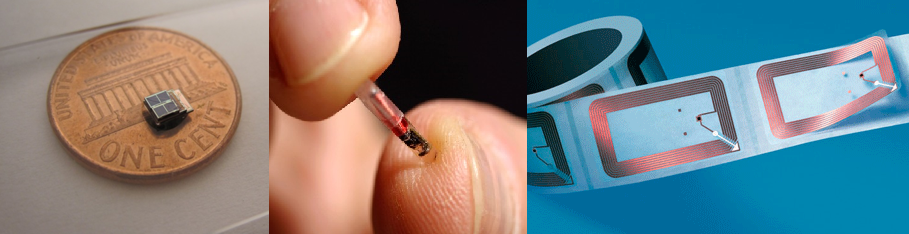
\includegraphics[width=15cm]{\rpDossier/images/capteurs.png}
\end{center}
\caption{Exemple de capteurs}
\label{conflinphone}
\end{figure}

Quelles seront les impacts et les possibilités de l'IoT ? Nous ne sommes limités seulement par notre imagination car nous changeons l'approche de voir et de connecter les objets.

Prenons quelques exemples pour montrer l'intérêt de l'IoT. Le \textit{monitoring} ne se résume pas qu'aux réseaux et machines, on peut aussi l'appliquer pour surveiller l'état d'un patient en médecine. Imaginons quelqu'un avec un problème cardiaque, il possède un pacemaker qui est "connecté", cela veut dire qu'une application sur son téléphone peut dire à cette personne l'état de son cœur, mais aussi à son hôpital. Dans le cas d'un défaillance, une alerte est lancée à l'hôpital qui peut envoyer immédiatement une ambulance, quand à la localisation ils peuvent utiliser un tracker GPS intégré au tout.

Grâce à des algorithmes puissant, on pourra même prédire un potentiel problème sans que le patient vienne faire des visites de contrôles régulières, son pacemaker enverra les données pour lui. Avec le nombre de personne de plus de 65 qui va doubler dans peu de temps, la e-santé et la télé-médecine vont devenir un des plus gros secteurs de l'IoT. 

Les tracas de quotidiens comme la perte de ses clefs ne seront plus un problème, en effet, dans le monde de l'IoT vos clés sont géo-localisables. Cela peut s'appliquer à plein de choses, si ce n'est à toutes, vous ne perdrez plus jamais rien.

Si nous savons où les choses sont et dans quelles états elles sont, nous pouvons mieux les manager. Prenons le cas du trafic en ville, si je sais où les voitures sont et ou elles vont, nous pouvons potentiellement éliminer les bouchons, optimiser les trajets et rediriger les flux plus facilement. Il en va de même pour l'énergie, si nous savons où l'énergie est requise, nous pouvons adapter la production et optimiser les coûts.

L'IoT permet aussi de déléguer du contrôle, toujours dans une optique d'optimisation énergétique, nous pouvons déléguer l'heure de départ d'une machine à laver, d'un lave-vaisselles à un contrôleur distant qui lancera le programme au moment où l'énergie sera la moins chère.

% Video-games

Un autre marché que l'IoT va investir est le jeux-vidéo.


% Privacy %

% Security %
% Partie 1.2 - Les différents protocoles %

\subsection{Les différents protocoles}
% Partie 1.3 - 6LoWPAN %

\subsection{6LoWPAN}


% Partie 3 - Bilan%

\section{Bilan}

\subsection{Travail accompli}

\subsection{Difficultés rencontrées}

\subsection{Perspectives}


\newpage

\sectionSpeciale{Conclusion}
% Conclusion du rapport

% Découverte IoT
Au travers de ce projet, nous avons pu découvrir le domaine de l’IoT et les perspectives que ces technologies offrent.
L’IoT n’est pour l’instant pas encore très présent dans notre vie courante mais pourrait vite le devenir.
Les constructeurs l’ont bien compris et sont particulièrement actif dans le développement de l’IoT, mais c’est à l’origine d’un manque d’uniformité qui ralentit paradoxalement cette évolution.

% Découverte d'un protocole pour l'IoT
Nous avons étudié l’un des protocoles de communication créé pour répondre aux problèmes de l’IoT, le 6LoWPAN.
Le manque de maturité des outils a freiné notre travail de recherche et de test, mais nous avons pu montrer la possibilité d’utiliser ce protocole.

% 


\newpage

%%% Après-propos %%%

% Changement des chiffres utilisés pour les numéros de pages
\pagenumbering{roman}
% Rétablissement du numéro de page méta
\setcounter{page}{\value{metapage}}

\ifdefined\rpWebographie
	\sectionSpeciale{Références}
	
	\bibliographie{Références bibliographiques}{bibliographie}
	\bibliographie{Références webographiques}{webographie}
\else
	\sectionSpeciale{Références bibliographiques}
	\bibliographieSansTitre{bibliographie}
\fi

\ifdefined\rpLexique
	\newpage
	\sectionSpeciale{\rpTitreLexique}
	
	\begin{description}[style=nextline]
		\input{contenu/lexique}
	\end{description}
\fi

% Annexes
\ifdefined\rpAnnexes
	\newpage
	\listeannexes
	\input{contenu/annexes}
\fi

\end{document}
